\documentclass[letterpaper,10pt,titlepage,draftclsnofoot,onecolumn,onesided] {IEEEtran}
\usepackage{listings}
\usepackage{underscore}
\usepackage[bookmarks=true]{hyperref}
\usepackage[utf8]{inputenc}
\usepackage[english]{babel}
%\usepackage{titling}
\usepackage{graphicx}
\usepackage{xcolor}
\usepackage[noadjust]{cite}
\usepackage{setspace}
\nocite{*}
\graphicspath{ {img/} }
%\usepackage{abstract}

\newcommand{\namesigdate}[2][4cm]{%
  \begin{tabular}{@{}p{#1}@{}}
    #2 \\[2\normalbaselineskip] \hrule \\[0pt]
    {\small \textit{Signature}} \\[2\normalbaselineskip] \hrule \\[0pt]
    {\small \textit{Date}}
  \end{tabular}
}
\newcommand{\studentnamesigdate}[2][4cm]{%
  \begin{tabular}{@{}p{#1}@{}}
    #2 \\[2\normalbaselineskip] \hrule \\[0pt]
    {\small \textit{Signature}} \\[2\normalbaselineskip] \hrule \\[0pt]
    {\small \textit{Signature}} \\[2\normalbaselineskip] \hrule \\[0pt]
    {\small \textit{Signature}} \\[2\normalbaselineskip] \hrule \\[0pt]
    {\small \textit{Signature}} \\[2\normalbaselineskip] \hrule \\[0pt]
    {\small \textit{Date}}
  \end{tabular}
}

\hypersetup{
    bookmarks=false,    % show bookmarks bar?
    pdftitle={Progress Report},    % title
    pdfauthor={Cramer Smith, Sam Lichlyter, Eric Winkler, Zach Schneider},                     % author
    pdfsubject={Progress Report},                        % subject of the document
    pdfkeywords={IFT, Report, Postal}, % list of keywords
    colorlinks=true,       % false: boxed links; true: colored links
    linkcolor=black,       % color of internal links
    citecolor=black,       % color of links to bibliography
    filecolor=black,        % color of file links
    urlcolor=blue,        % color of external links
    linktoc=page            % only page is linked
} 

\lstdefinestyle{customperl}{
  belowcaptionskip=1\baselineskip,
  breaklines=true,
  frame=L,
  xleftmargin=\parindent,
  language=Perl,
  columns=fullflexible,
  showstringspaces=false,
  basicstyle=\footnotesize\ttfamily,
  keywordstyle=\bfseries\color{green!40!black},
  commentstyle=\itshape\color{purple!40!black},
  identifierstyle=\color{blue},
  stringstyle=\color{orange},
  numbers=left
}
\lstset{escapechar=@, style=customperl}

% Document Title:
\def\doctitle{A Tool to Automatically Organize the Structure of a Codebase Using Information Foraging Theory Design Patterns}
\def\doctype{Progress Report}
\def\doctype{Winter Midterm Update}
\def\team{Team Postal | Group \#38}

\markboth{Oregon State University}{\doctitle}

\begin{document}

\title{\Huge{\bfseries{\textsf{\doctitle}}}\\\textsf{\Large{\doctype}}\\\textsf{\large{\team}}}
\author{Cramer Smith, Sam Lichlyter, Eric Winkler, Zach Schneider}

\maketitle
\vfill

\vfill

\pagebreak

\tableofcontents


\pagebreak

\section{Project Purpose and Goals}
Developer tools are often complex pieces of software. 
Gathering and manipulating useful information for a programmer can often be a slow and costly process. 
By implementing Information Foraging Theory design patterns in the creation of these tools, the information collected may be more useful or obtained faster. 
Information Foraging Theory (IFT) is the theory and math behind the choices people make to maximize the value of the information they find versus the cost of getting that information.
The aim of this project is to develop a tool that will act as a proof of concept for IFT and increase developer efficiency.

The Postal extension is being designed to allow developers to more quickly search through and better visualize their projects.
This extension will also help developers create clearer and cleaner code structure by offering reminders and suggestions about the best coding practices in the programming language they are currently using.
Any major errors or incompatibilities within the project or its files will be reported to the developer as well.

\section{Current Status: Fall Term}

As of the end of Fall term, the Postal team has completed all documents and preliminary requirements needed to move forward with the creation of the Postal extension. 
Initial prototypes for both UI elements and file parsing components of the extension exist and are beginning to be further developed. 
The team aims to have a fully working prototype by the end of Winter break that is able to parse and display any web development project.
Current and prior progress indicates that the Postal team is on track to meet this self and client imposed deadline.
Below are current descriptions and functionalities provided by the major components within the Postal extension.

\subsection{Parsers}
The current implementation of the extension has one parser which parses HTML.
This parser is implemented in Perl using the Simple TokeParser which looks for specific tags and a specific attribute from that tag.
For example, this HTML parser specifically looks for the anchor (\verb|a|) tag and the hyperlink reference (\verb|href|) attribute and returns those values which are the links to either outside websites or internal pages.

\subsection{User Interface}
The user interface is currently running off of dummy, static data. 
It opens up in a new window using a program called Electron as opposed to a web browser to cut down on the overhead associated with all the complexities of the web browser.
It shows each web page as a node and each link from one page to another as an edge in a graph. See Figure 1.
\begin{figure}
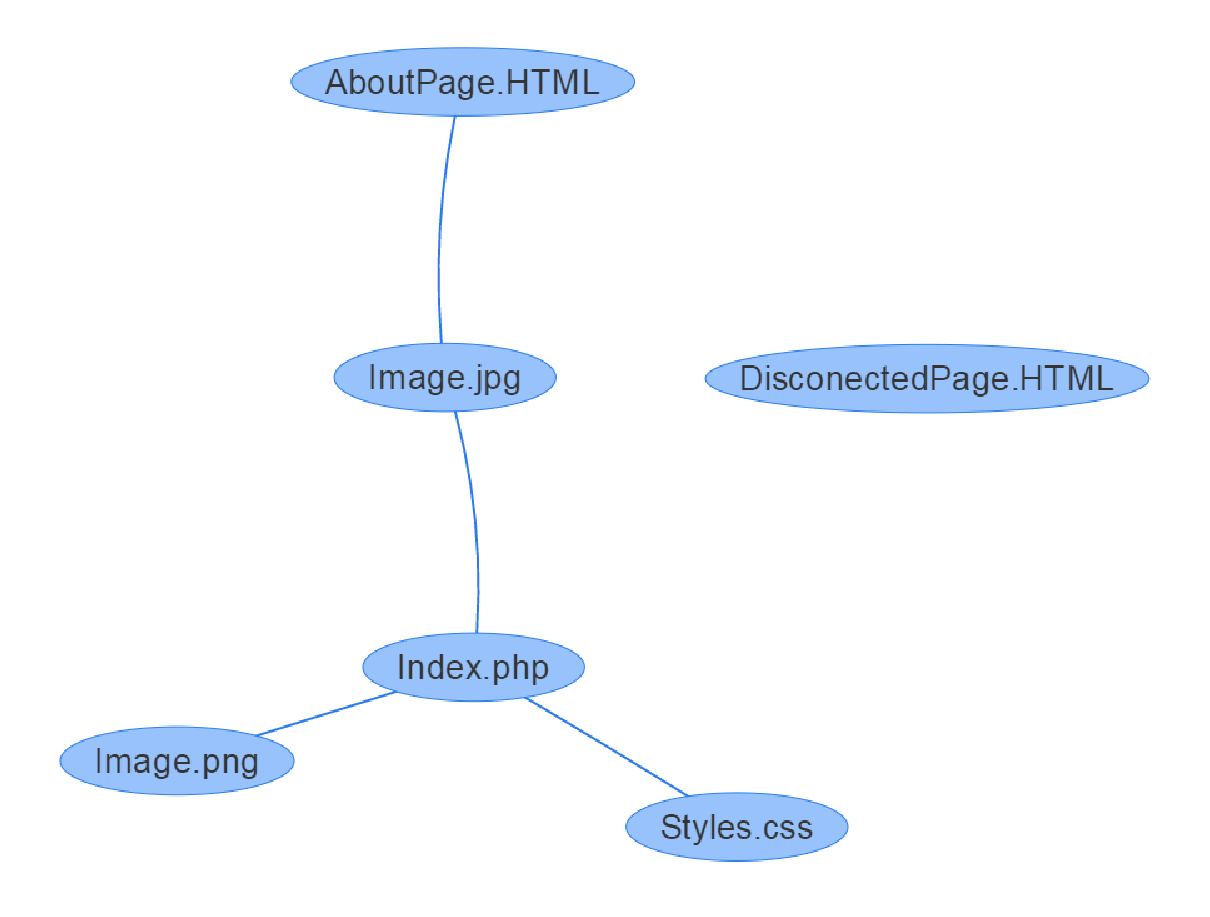
\includegraphics[width=300px]{UIMockupEPS}
\caption{User Interface Example}
\end{figure}

\subsection{Data Layer}
The data layer is comprised of a data structure and data access methods.
The data structure is defined below in the ERD (Figure 2).
\begin{figure}
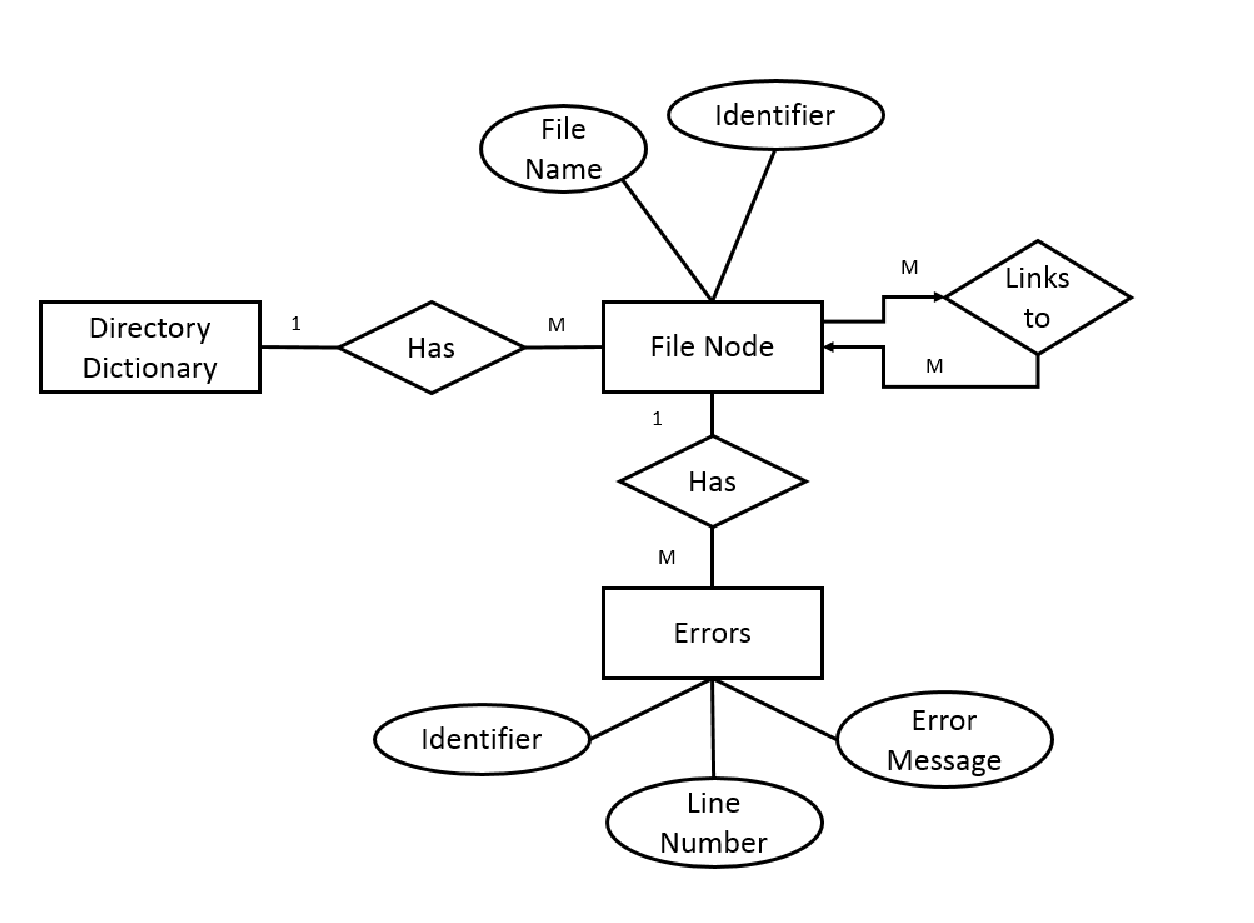
\includegraphics[width=300px]{InformationERDEPS}
\caption{Data Structure ERD}
\end{figure}

\section{Problems and Solutions: Fall Term}
	\subsection{Pre-Week 3}
	The beginning of our project was back in August when Sam told the rest of the team about an opportunity that he had to work with Prof. Chirs Scaffidi on a senior design project. 
	The members of the team all jumped on the opportunity to work together for a professor all of us had had previously and throughly enjoyed.
	Prof. Scaffidi tasked the team with coming up with project proposals.
	The only requirements for the project is that it had to be a tool that used information foraging theory to do anything.
	The first problem was that none of the team knew what IFT was so the team took a week to brainstorm seperately and research IFT and come up with project ideas.
	After that week the team met and decided on two ideas to give to the client.
	Scaffidi chose a code base organization tool that would be an extension for Visual Studio Code.
	
	\subsection{Week 3}
	After the first couple weeks of class while other teams were just meeting the Postal team was able to start meeting and thinking about functionality as well as begin to work on the problem statement.
	The problem statement was the first document of the project and it was a challenge to create an official document and learn how to use the IEEE standard. 
	This problem was not really solved.
	The team ended up creating what they thought was a good document, and there was feedback on the document that came later in the quarter helped tremendously for the next draft of the document.
	
	\subsection{Week 4}
	During the fourth week, our client had challenged the team with accelerating the development process past the class.
	In response to this request the team started developing basic "hello world" extensions with very limited to no functionality.
	These programs served as a learning experience for the team as we develop more complex extensions these examples gave us a framework of understanding of what the code of an extension looks like.
	These small programs were good but not up to par with our clients expectations.	
	
	\subsection{Week 5}
	In week five the team revised the problem statement.
	This task was fairly easy as the team had received feedback on the first draft and therefore had a knowledge of what was expected of them.
	This week we also started work on the Requirements Document. 
	The requirements document was much more daunting than the problem statement as it was more technical, and made the team think more the project as a piece of software an not just a problem to be solved.
	The team wrote a first draft of the requirements document and made a plan to finish it the next week.
	
	\subsection{Week 6}
	With the completion of the requirements document the team had some solid ideas as to what the project was going to look like.
	This was a big step forward for the project as the team had only a fuzzy idea as to what the project really looked like at this moment.
	Now the team knew that it was going to be a web development tool instead of a general code organizer.
	This was great for the development of the project, but this narrowing of scope was not communicated to the client. 
	The team thought that they had communicated this in a meeting but apparently either our client did not understand or the idea was not stated clearly.
	This caused problems later in the process.
	
	\subsection{Week 7}
	This week we thought was a big step for the team. 
 	By this time there was a working prototype of the user interface, and a simple parser for HTML.
	The only thing was that these programs were not actually a Visual Studio Code extension but separately compiled programs.
	The team needed to figure out how to combine the program UI with Visual Studio Code.
	
	\subsection{Week 8}
	The eighth week the team finished the tech document.
	The tech document made the team look at alternatives for parts that each member had decided to focus on.
	This was eye opening as we researched alternatives to pieces of the project that the team members had never thought of before.
	
	\subsection{Week 9}
	This week was Thanksgiving week. 
	With the extra time Sam and Eric were able to further the prototype and make some small improvements.
	These small improvements still had not added the UI to the extension but the team thought that it would be good enough to show to the client. 

	\subsection{Week 10}
	Week ten was a big week as the design document was due that week. 
	This document proved to be the most confusing as the team had a particularly difficult time figuring out the IEEE standard of the software design document. 
	The team was able to struggle through the design document and create what the team thought was good document. 
	The team also was able to show to the client what we had done with the prototype so far. 
	The client was happy with the prototype, but encouraged the team to reconsider the reduction in scope that had occured previously.
	This will be factored into the work going forward.
	
\section{Prototype Code Samples}
	
	\subsection{FileMap UI}
	\begin{lstlisting}

	\end{lstlisting}

	\subsection{HTML Parser}
	\begin{lstlisting}
my $anchor_parser = HTML::TokeParser::Simple->new(handle => *DATA);
while (my $anchor = $anchor_parser->get_tag('a')) {
    next unless defined(my $href = $anchor->get_attr('href'));
    say $href;
}
	\end{lstlisting}
	
\pagebreak
\section{Fall Term Retrospective}
	\begin{center}
	\begin{singlespace}
		\begin{tabular}{ |  p{0.25\linewidth}  |  p{0.25\linewidth}  | p{0.25\linewidth} | p{0.25\linewidth} |}
		\hline
		Topic & Positives & Deltas & Actions \\ \hline
		
			Communication with client 
		& 
			\begin{itemize}
				\item Flexible in terms of project requirements.
				\item Provided the team with a mock up application architecture.
				\item Easy to work with.
			\end{itemize}
		& 
			\begin{itemize}
				\item Frequency and clarity of communication need to be improved.
			\end{itemize}
		&
			\begin{itemize}
				\item Solidify team member responsibilities (Sam is in charge of emailing the client).
				\item The team as a whole will need to make sure Sam is aware of things that need to be communicated with the client.
			\end{itemize} 
		\\ \hline
			Team Effectiveness 
		& 
			\begin{itemize}
				\item Members have flexible schedules and are easy to sit down with.
				\item Members all do a good job of quickly replying to communications.
				\item Members have a positive attitude.
			\end{itemize}
		& 
			\begin{itemize}
				\item As a team, assignments do not get much planning and are usually done last minute.
				\item There is no clear team leader.
			\end{itemize}
		&
			\begin{itemize}
				\item Assign a pseudo team leader with the responsibility of tracking/ scheduling tasks and work assignments.
			\end{itemize} 
		\\ \hline
			Implementation 
		& 
			\begin{itemize}
				\item The team has become much more capable at developing with the VSC IDE.
				\item The Team has already built a couple of working prototypes for the client.
			\end{itemize}
		& 
			\begin{itemize}
				\item The Gantt chart is currently out of date and needs updating.
				\item Some technical implementation obstacles have yet to be addressed (npm auto installing).
			\end{itemize}
		&
			\begin{itemize}
				\item Update Gantt chart to better reflect the current progress and set new goal deadlines for winter term.
			\end{itemize} 
		\\ \hline
			Design 
		& 
			\begin{itemize}
				\item The current design meets requirements and team members are aware of their design related responsibilities.
			\end{itemize}
		& 
			\begin{itemize}
				\item IFT Design Pattern tie-ins are not 100\% clear and as a major requirement of the project, they need to be.
				\item Parse needs to be redesigned to better match our scope. See Week 10 notes.
			\end{itemize}
		&
			\begin{itemize}
				\item The team will need to meet to re-design the parser component of the extension and review the selected IFT design patterns.
			\end{itemize} 
		\\ \hline
			Documentation 
		& 
			\begin{itemize}
				\item All assigned documentation is currently in a workable state.
			\end{itemize}
		& 
			\begin{itemize}
				\item Team members feel that the documentation is typically rushed and not a descriptive as it should be.
				\item Team members have a difficult time interpreting the IEEE standards and thi may be a partial cause to the above.
			\end{itemize}
		&
			\begin{itemize}
				\item A team member will take a leadership position to schedule work tasks which will ensure that the team has sufficient time to complete the documentation assignments to a higher standard. 
			\end{itemize} 
		\\ \hline
		\end{tabular}
		\end{singlespace}
	\end{center}

\section{Current Status: Winter Midterm Update}
%%Add status as off week 7

	\subsection{Parser}

	\subsection{User Interface}

	\subsection{Data Layer}

\section{Problems and Solutions: Winter Midterm }
	\subsection{Winter Break}

	\subsection{Week 1}

	\subsection{Week 2}

	\subsection{Week 3}

	\subsection{Week 4}

	\subsection{Week 5}

	\subsection{Week 6}

\section{Prototype Code Samples}	

\pagebreak
\section{Winter Midterm Retrospective}
	\begin{center}
	\begin{singlespace}
		\begin{tabular}{ |  p{0.25\linewidth}  |  p{0.25\linewidth}  | p{0.25\linewidth} | p{0.25\linewidth} |}
		\hline
		Topic & Positives & Deltas & Actions \\ \hline
		
			Communication with client 
		& 
			\begin{itemize}
				\item 
			\end{itemize}
		& 
			\begin{itemize}
				\item 
			\end{itemize}
		&
			\begin{itemize}
				\item 
			\end{itemize} 
		\\ \hline
			Team Effectiveness 
		& 
			\begin{itemize}
				\item 
			\end{itemize}
		& 
			\begin{itemize}
				\item 
			\end{itemize}
		&
			\begin{itemize}
				\item 
			\end{itemize} 
		\\ \hline
			Implementation 
		& 
			\begin{itemize}
				\item .
			\end{itemize}
		& 
			\begin{itemize}
				\item 
			\end{itemize}
		&
			\begin{itemize}
				\item 
			\end{itemize} 
		\\ \hline
			Design 
		& 
			\begin{itemize}
				\item 
			\end{itemize}
		& 
			\begin{itemize}
				\item 
			\end{itemize}
		&
			\begin{itemize}
				\item 
			\end{itemize} 
		\\ \hline
			Documentation 
		& 
			\begin{itemize}
				\item 
			\end{itemize}
		& 
			\begin{itemize}
				\item 
			\end{itemize}
		&
			\begin{itemize}
				\item 
			\end{itemize} 
		\\ \hline
		\end{tabular}
		\end{singlespace}
	\end{center}

\pagebreak
\bibliographystyle{IEEEtran}
\bibliography{progress-report-team38}

\end{document}